\section{Polar Coordinates}
  In addition to Cartisian coordinates, we can also use a \textbf{polar coordinate system}.
  \begin{center}
    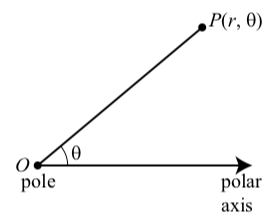
\includegraphics[width=150pt]{polar.png}
  \end{center}
  Point $P$ is represented by the ordered pair $(r,\theta)$, where $r$ is the distance to the point from the center and $\theta$ is the angle from the polar axis to the point.
  \par
  The points $(r,\theta)$ and $(-r,\theta)$ are on the same line and have the same distance $|r|$ from the center but are on opposite sides of the center. Additionally, $(-r,\theta)$ and $(r,\theta+\pi)$ are also on the same line.
  \par
  This means a complete counterclockwise rotation is given by an angle $2\pi$, so $(r,\theta)$ is also represented by
  \begin{center}
    $(r,\theta+2n\pi)$ and $(-r,\theta+(2n+1)\pi)$
  \end{center}
  \subsection*{Relationship Between Cartesian and Polar Coordinates}
    \begin{center}
      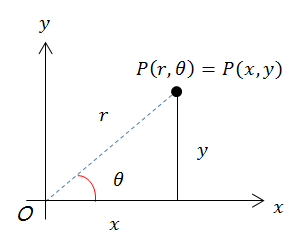
\includegraphics[width=150pt]{cartesian_to_polar.png} \\
      $\cos\theta = \frac{x}{r}$\ \ \ $\sin\theta = \frac{y}{r}$ \\~\\
      $x=r\cos\theta$ \ \ \  $y=r\sin\theta$ \\~\\
      $r^2 = x^2 + y^2$ \ \ \  $\tan\theta = \frac{y}{x}$
    \end{center}
    \begin{example}
      Convert the point $(2,\pi/3)$ from polar to Cartesian coordinates.
    \end{example}
    \begin{solution}
      \begin{align*}
        r=2,\ \theta=\pi/3 \\
        x&=r\cos\theta = 2\cos\frac{\pi}{3}=2\cdot\frac{1}{2}=1 \\
        y&=r\sin\theta = 2\sin\frac{\pi}{3}=2\cdot\frac{\sqrt{3}}{2}=\sqrt{3}
      \end{align*}
      So the point is $(1,\sqrt{3})$ in Cartesian coordinates.
    \end{solution}
    \begin{example}
      Represent the Cartesian coordinates $(1,-1)$ in polar coordinates.
    \end{example}
    \begin{solution}
      \begin{align*}
        r&=\sqrt{x^2 + y^2}=\sqrt{1^2 + (-1)^2} = \sqrt{2} \\
        \tan\theta &= \frac{y}{x} = -1
      \end{align*}
      Since the point (1,-1) lies in the fourth quadrant, we can choose $\theta=-pi/4$ or $\theta=7pi/4$. So the possible answers are either $(\sqrt{2},-\pi/4$ or $(\sqrt{2},7\pi/4$.
    \end{solution}
  \subsection*{Polar Curves}
    The \textbf{graph of a polar equation} $r=f(\theta)$, or $F(r,\theta) = 0$, consists of all of the points where $(r,\theta)$ satisfies the equation.
  \subsection*{Tangents to Polar Curves}
    To find a tangent line to a polar curce $r=f(\theta)$, we regard $\theta$ as a parameter and write the parametric equations as
    \begin{center}
      $x=r\cos\theta = f(\theta)\cos\theta$\ \ \ $y=r\sin\theta=f(\theta)\sin\theta$
    \end{center}
    So
    \begin{definition}
      \begin{equation*}
        \frac{dy}{dx}=\frac{\frac{dy}{d\theta}}{\frac{dx}{d\theta}} = \frac{\frac{dy}{d\theta}sin\theta+r\cos\theta}{\frac{dr}{d\theta}\cos\theta-r\sin\theta}
      \end{equation*}
    \end{definition}

    \begin{itemize}
      \item horizontal tangent when $ \frac{dy}{d\theta} = 0 $ (provided that $\frac{dx}{d\theta} \neq 0$)
      \item vertical tangent when $ \frac{dx}{d\theta} = 0 $ (provided that $\frac{dy}{d\theta} \neq 0$)
    \end{itemize}
    \textsc{Note} tangent lines at the pole have r=0 and the slope of the tangent simplifies to
    \begin{equation*}
       \frac{dy}{dx}=\tan\theta \text{ if } \frac{dr}{d\theta} \neq 0
    \end{equation*}
    \begin{example}
      For the cardiod $r=1+\sin\theta$, find the slope of the tangent line when r=3
    \end{example}
    \begin{solution}
      \begin{align*}
        r &= 1+\sin\theta \\
        \frac{dy}{dx} &= \frac{\frac{dy}{d\theta}sin\theta+r\cos\theta}{\frac{dr}{d\theta}\cos\theta-r\sin\theta}
          = \frac{\cos\theta\sin\theta+(1+\sin\theta)\cos\theta}{\cos\theta\cos\theta-(1+\sin\theta)\sin\theta} \\
          &= \frac{\cos\theta(1+2\sin\theta)}{1-2\sin^2 \theta-\sin\theta}
          =\frac{\cos\theta(1+2\sin\theta)}{(1+\sin\theta)(1-\sin\theta)} \\
        \intertext{The slope of the tangent where $\theta=\pi/3$ is}  \\
        \frac{dy}{dx}\biggm\rvert_{\theta=\pi/3} &= \frac{\cos(\pi/3)(1+2\sin(\pi/3))}{(1+\sin(\pi/3))(1-\sin(\pi/3))} \\
          &= \frac{\frac{1}{2}(1+\sqrt{3})}{(1+\sqrt{3}/2)(1-\sqrt{3})} = \frac{1+\sqrt{3}}{(2+\sqrt{3})(1-\sqrt{3})} \\
          &= \frac{1+\sqrt{3}}{-1-\sqrt{3}} = -1
      \end{align*}
      \textsc{Note} Instead of memorizing the equation, we can instead use the same method we used to derive it.
      \begin{align*}
        x &= r\cos\theta = (1+\sin\theta)\cos\theta = \cos\theta+\frac{1}{2}\sin2\theta \\
        y &= r\sin\theta = (1+\sin\theta)\sin\theta = \sin\theta+\sin^2 \theta \\
        \frac{dy}{dx} &= \frac{dy/d\theta}{dx/d\theta} = \frac{cos\theta+2\sin\theta\cos\theta}{-\sin\theta+\cos2\theta} = \frac{\cos\theta+\sin2\theta}{-\sin\theta+\cos2\theta}
      \end{align*}
      This is equivalent to the previous equation.
    \end{solution}


